\documentclass[11pt,a4paper]{article}
\usepackage[T1]{fontenc}
\usepackage[utf8]{inputenc}
\usepackage{lmodern,microtype}
\usepackage[margin=21mm,headheight=15pt]{geometry}
\usepackage{amsmath,amssymb,booktabs,tabularx,array,enumitem}
\usepackage{xcolor,tikz,fancyhdr,titlesec,hyperref,graphicx}
\usetikzlibrary{arrows.meta,positioning,calc}
\definecolor{navy}{HTML}{193B54}
\definecolor{teal}{HTML}{087E8B}
\definecolor{pale}{HTML}{EDF6F6}
\definecolor{graycell}{HTML}{DCE1E5}
\hypersetup{colorlinks=true,linkcolor=navy,urlcolor=teal,citecolor=teal,
  pdftitle={Spatial EEGNet and spatial Transformer: a reproducible candidate study},
  pdfauthor={AGFL-inm research documentation}}
\pagestyle{fancy}\fancyhf{}
\fancyhead[L]{\small\textcolor{navy}{AGFL-inm\quad Spatial model guide}}
\fancyhead[R]{\small 3 October 2026}
\fancyfoot[C]{\thepage}
\setlength{\parindent}{0pt}\setlength{\parskip}{4pt}
\titlespacing*{\section}{0pt}{10pt}{6pt}
\titlespacing*{\subsection}{0pt}{8pt}{4pt}
\setlist{itemsep=3pt,topsep=4pt,leftmargin=*}
\renewcommand{\arraystretch}{1.12}
\newcolumntype{Y}{>{\raggedright\arraybackslash}X}
\newcolumntype{L}[1]{>{\raggedright\arraybackslash}p{#1}}
\newcommand{\code}[1]{{\small\nolinkurl{#1}}}
\newcommand{\takeaway}[1]{\par\smallskip\noindent\fcolorbox{teal}{pale}{%
  \parbox{\dimexpr\linewidth-2\fboxsep-2\fboxrule\relax}{#1}}\par\smallskip}
\tikzset{box/.style={draw=teal,fill=pale,rounded corners=2pt,align=center,
  text width=36mm,minimum height=13mm,font=\small,inner sep=4pt},
  smallbox/.style={draw=teal,fill=pale,rounded corners=2pt,align=center,
  text width=28mm,minimum height=12mm,font=\small,inner sep=3pt},
  arrow/.style={-{Latex[length=2mm]},thick,draw=navy}}

\begin{document}
{\LARGE\bfseries\color{navy} Spatial EEGNet and spatial Transformer}\par
{\large A teaching guide to the reproducible candidate cohort}\par
\textbf{Scope.} Two end-to-end raw-EEG classifiers in the separate
\code{encoder_candidates} study: \code{spatial_eegnet} and
\code{spatial_transformer}. This guide follows the real, frozen reproducible-v1
cohort. Both systems classify four motor-imagery classes for one participant
at a time. The name ``spatial Transformer'' refers to its EEGNet spatial
front end; the Transformer attention itself is over a short temporal sequence.

\section{The models at a glance}
The question is whether replacing EEGNet's flattened temporal readout with one
small Transformer encoder layer changes clean validation performance. The
front end first mixes electrode signals into learned features. The Transformer
then relates 31 time positions in those features. Neither arm uses the legacy
Tucker representation or attention over 22 electrode tokens.

\begin{center}
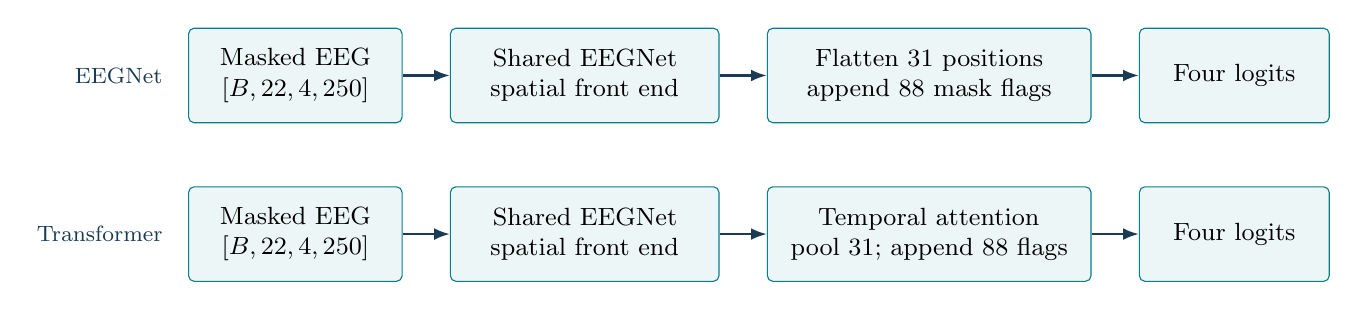
\begin{tikzpicture}[node distance=5mm and 6mm]
\node[smallbox,text width=25mm] (d1) {Masked EEG\\$[B,22,4,250]$};
\node[smallbox,text width=32mm,right=of d1] (f1) {Shared EEGNet\\spatial front end};
\node[smallbox,text width=39mm,right=of f1] (r1) {Flatten 31 positions\\append 88 mask flags};
\node[smallbox,text width=22mm,right=of r1] (o1) {Four logits};
\node[smallbox,text width=25mm,below=8mm of d1] (d2) {Masked EEG\\$[B,22,4,250]$};
\node[smallbox,text width=32mm,right=of d2] (f2) {Shared EEGNet\\spatial front end};
\node[smallbox,text width=39mm,right=of f2] (r2) {Temporal attention\\pool 31; append 88 flags};
\node[smallbox,text width=22mm,right=of r2] (o2) {Four logits};
\draw[arrow] (d1)--(f1);\draw[arrow] (f1)--(r1);\draw[arrow] (r1)--(o1);
\draw[arrow] (d2)--(f2);\draw[arrow] (f2)--(r2);\draw[arrow] (r2)--(o2);
\node[left=2mm of d1,font=\footnotesize\color{navy},anchor=east] {EEGNet};
\node[left=2mm of d2,font=\footnotesize\color{navy},anchor=east] {Transformer};
\end{tikzpicture}
\end{center}

\begin{tabularx}{\linewidth}{@{}L{37mm}YY@{}}
\toprule
Property & \code{spatial_eegnet} & \code{spatial_transformer} \\
\midrule
Shared front end & EEGNet temporal, spatial, and separable convolutions & Same modules and identical initialization for a given seed \\
Readout sequence & $[B,31,16]$, flattened to 496 values & Project to $[B,31,32]$, one temporal Transformer layer, mean pool \\
Availability input & 88 Boolean channel-window flags & Same 88 flags after temporal pooling \\
Trainable parameters & 3,796 & 11,092 \\
Role in comparison & Reference arm & Complete alternate head, not an isolated attention ablation \\
\bottomrule
\end{tabularx}

\takeaway{\textbf{Read the word ``spatial'' carefully.} EEGNet's depthwise
convolution spans the 22-electrode axis. Once that operation runs, its 16
feature maps are learned mixtures, not individually identifiable electrodes.
The Transformer applies self-attention over the 31 pooled temporal positions.}

\textbf{Reading map.} Sections 2--4 trace the inputs and both architectures;
section 5 explains loss and evaluation; sections 6--7 cover results, prior
models, and novelty; section 8 records provenance and source locations.

\newpage
\section{Dataset, trial construction, and normalization}
\subsection*{One example}
The cohort uses BCI Competition IV dataset 2a: nine participants, four
classes (left hand, right hand, feet, tongue), 22 EEG electrodes, sampled at
250 Hz. The default files are the participants' T-session recordings. A trial
starts at the class cue and contains 1,000 samples, or four seconds. Artifact
marked, out-of-bounds, or nonfinite trials are excluded by the loader; counts
are recorded in provenance. The canonical signal before windowing is
$[N,22,1000]$, with integer label $y\in\{0,1,2,3\}$.

\begin{tabularx}{\linewidth}{@{}L{42mm}Y@{}}
\toprule
Stage & Operation and resulting shape \\
\midrule
Read & Accepted cue-aligned EEG: $[N,22,1000]$ \\
Filter & 2--30 Hz Butterworth SOS, order argument 4, forward--backward; each electrode and one-second window filtered separately \\
Window & Split the 1,000 samples into four adjacent windows of 250 samples: $[N,22,4,250]$ \\
Normalize & Training-trial/channel/time mean and population standard deviation; standard deviation floor $10^{-8}$ \\
Input & Float tensor $X\in\mathbb R^{B\times22\times4\times250}$ \\
Mask & Boolean availability $M\in\{0,1\}^{B\times22\times4}$; 1 means present in that whole one-second window \\
Output & Four unnormalized class scores (logits), shape $[B,4]$ \\
\bottomrule
\end{tabularx}

For each channel $c$, the training partition alone determines
\[
 \mu_c=\frac{1}{|\mathcal T|1000}\sum_{i\in\mathcal T,t}R_{ict},\qquad
 \sigma_c=\max\left(\sqrt{\frac{1}{|\mathcal T|1000}
 \sum_{i\in\mathcal T,t}(R_{ict}-\mu_c)^2},10^{-8}\right),
 \quad X_{ict}=\frac{R_{ict}-\mu_c}{\sigma_c}.
\]
The saved training statistics are applied unchanged to validation. Samples are
split within each participant and T session, approximately 60\% train, 20\%
validation, and 20\% held out, stratified by class for each seed. There are
nine participants and three seeds, or 27 paired participant/seed tasks.

\subsection*{Removing unavailable values safely}
Before any convolution or channel mixing, the models select observed values:
\[
 \widetilde X_{bcp\tau}=\begin{cases}
 X_{bcp\tau},&M_{bcp}=1,\\0,&M_{bcp}=0.
 \end{cases}
\]
The implementation uses \code{torch.where}. This matters if a hidden entry is
NaN: multiplying it by zero still leaves NaN. A zero after normalization is
the training mean value in raw units. Each trial/window must retain at least
one electrode.

\takeaway{Training is \textbf{full input only}: every one of the 88 flags is
1 during optimization and epoch selection. Masked validation conditions are
diagnostics. Passing a mask to the model does not by itself train robustness
to missing electrodes.}

\newpage
\section{Model 1: the mask-conditioned spatial EEGNet}
This arm wraps the project's EEGNet classifier with fixed settings
$F_1=8$, depth multiplier $D=2$, and $F_2=16$. The implementation follows
EEGNet's compact temporal / depthwise spatial / separable convolution pattern
\cite{eegnet}. It learns all filters and the classifier together by class
cross-entropy.

\begin{center}
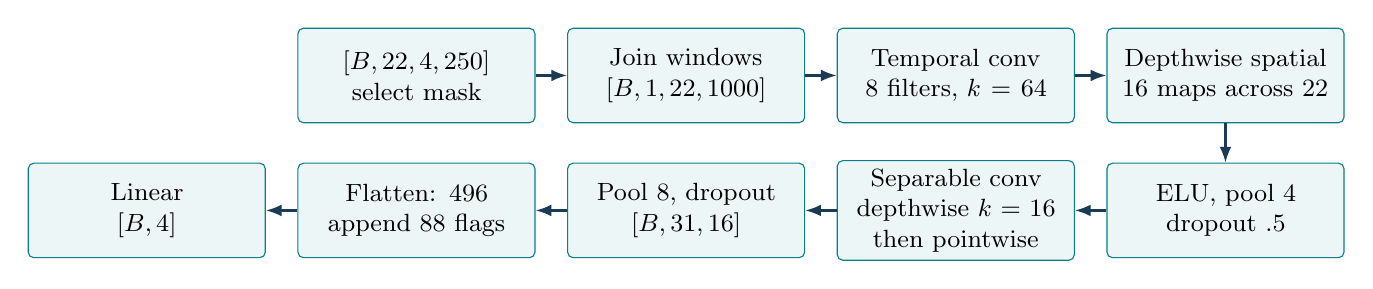
\begin{tikzpicture}[node distance=5mm and 4mm]
\node[smallbox] (in) {$[B,22,4,250]$\\select mask};
\node[smallbox,right=of in] (reshape) {Join windows\\$[B,1,22,1000]$};
\node[smallbox,right=of reshape] (temp) {Temporal conv\\8 filters, $k=64$};
\node[smallbox,right=of temp] (spat) {Depthwise spatial\\16 maps across 22};
\node[smallbox,below=of spat] (pool1) {ELU, pool 4\\dropout .5};
\node[smallbox,left=of pool1] (sep) {Separable conv\\depthwise $k=16$\\then pointwise};
\node[smallbox,left=of sep] (pool2) {Pool 8, dropout\\$[B,31,16]$};
\node[smallbox,left=of pool2] (flat) {Flatten: 496\\append 88 flags};
\node[smallbox,left=of flat] (logits) {Linear\\$[B,4]$};
\draw[arrow] (in)--(reshape);\draw[arrow] (reshape)--(temp);
\draw[arrow] (temp)--(spat);\draw[arrow] (spat)--(pool1);
\draw[arrow] (pool1)--(sep);\draw[arrow] (sep)--(pool2);
\draw[arrow] (pool2)--(flat);\draw[arrow] (flat)--(logits);
\end{tikzpicture}
\end{center}

\subsection*{Shapes and purpose}
\begin{tabularx}{\linewidth}{@{}L{45mm}L{34mm}Y@{}}
\toprule
Operation & Output & Interpretation \\
\midrule
Select mask, reshape & $B\times1\times22\times1000$ & Four adjacent windows are rejoined before learned convolution \\
Temporal conv + BatchNorm & $B\times8\times22\times1000$ & Length-64 filters run at every electrode \\
Depthwise spatial conv + BN & $B\times16\times1\times1000$ & Two electrode-spanning filters per temporal map \\
ELU, average pool 4, dropout & $B\times16\times1\times250$ & Nonlinearity and first time reduction \\
Depthwise temporal conv $k=16$, pointwise mix, BN & $B\times16\times1\times250$ & Temporal refinement, then mix feature maps \\
ELU, average pool 8, dropout & $B\times16\times1\times31$ & Ordered temporal summary positions \\
Squeeze and transpose & $B\times31\times16$ & Time-major sequence exposed by \code{forward_features} \\
Flatten + 88 flags & $B\times584$ & $31\cdot16+22\cdot4$ classifier inputs \\
Linear & $B\times4$ & Four class logits \\
\bottomrule
\end{tabularx}

The convolutions use padding that preserves time length before pooling. The
temporal filters run over the concatenated 1,000-sample sequence with kernel
width 64. Filtering is window-local, but the learned convolution can mix
information across the joins between windows. The spatial convolution
collapses the electrode axis; it does not produce one output token per
electrode. Dropout rate is 0.5. After each optimizer step, the EEGNet arm
clips spatial-filter max norm to 1.0 and final-classifier row max norm to 0.25.

The mask is flattened in canonical electrode-then-window order and appended
after the 496 signal values. Since training masks are all ones, this head
learns with a constant availability vector during fitting. At masked
evaluation, the vector informs the classifier which inputs were zeroed, while
the front-end filters still see those zeros.

\newpage
\section{Model 2: EEGNet front end plus a compact temporal Transformer}
The arm constructs the exact EEGNet initialization for a given seed and keeps
its convolutional feature layers. The EEGNet arm and Transformer arm therefore
start with identical front-end tensors. They then optimize independently; the
shared start is not a frozen feature extractor.

\begin{center}
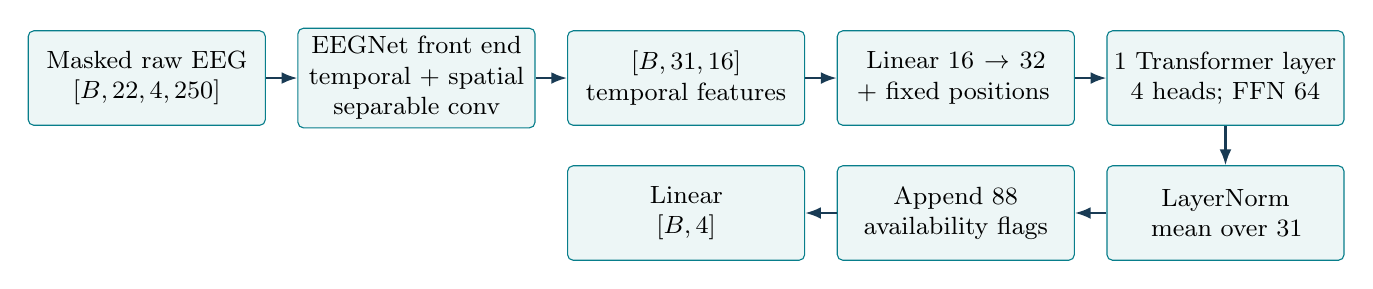
\begin{tikzpicture}[node distance=5mm and 4mm]
\node[smallbox] (raw) {Masked raw EEG\\$[B,22,4,250]$};
\node[smallbox,right=of raw] (front) {EEGNet front end\\temporal + spatial\\separable conv};
\node[smallbox,right=of front] (seq) {$[B,31,16]$\\temporal features};
\node[smallbox,right=of seq] (proj) {Linear $16\to32$\\+ fixed positions};
\node[smallbox,right=of proj] (trans) {1 Transformer layer\\4 heads; FFN 64};
\node[smallbox,below=of trans] (norm) {LayerNorm\\mean over 31};
\node[smallbox,left=of norm] (flags) {Append 88\\availability flags};
\node[smallbox,left=of flags] (out) {Linear\\$[B,4]$};
\draw[arrow] (raw)--(front);\draw[arrow] (front)--(seq);
\draw[arrow] (seq)--(proj);\draw[arrow] (proj)--(trans);
\draw[arrow] (trans)--(norm);\draw[arrow] (norm)--(flags);
\draw[arrow] (flags)--(out);
\end{tikzpicture}
\end{center}

\subsection*{Temporal positions and self-attention}
Each of the 31 front-end positions has 16 values. A learned linear map gives
32 values, then a fixed sinusoidal position code is added. This tells the
attention layer which temporal position a vector came from. One batch-first,
pre-layer-normalized encoder layer uses four attention heads, a 64-wide GELU
feed-forward sublayer, and dropout 0.1. A final LayerNorm is applied before
averaging positions. The result is 32 values; appending the same 88 flags
gives 120 inputs to the class layer.

For one attention head, the scaled dot-product operation is
\[
 \operatorname{Attn}(Q,K,V)=
 \operatorname{softmax}\!\left(\frac{QK^\top}{\sqrt{d_k}}\right)V,
 \qquad Q=XW_Q,\;K=XW_K,\;V=XW_V.
\]
Here rows of $X$ are time positions (31 rows), not electrodes. Multi-head
attention computes this with four learned projections, combines the head
outputs, and uses residual connections and layer normalization. The PyTorch
encoder layer also contains the position-wise feed-forward block
\[
 \operatorname{FFN}(x)=W_2\,\operatorname{GELU}(W_1x+b_1)+b_2,
 \quad 32\to64\to32.
\]
With pre-normalization, each sublayer adds its input through a residual path.
The Transformer output sequence remains $[B,31,32]$ until mean pooling. Its
training step clips shared spatial filters to max norm 1.0 but does not clip
the final classifier; this is one regularization difference from EEGNet.

\begin{tabularx}{\linewidth}{@{}L{47mm}Y@{}}
\toprule
Setting & Declared value \\
\midrule
Projection width / position code & $16\to32$ / fixed sinusoidal for positions 0--30 \\
Encoder & One layer; four heads; batch-first; norm-first \\
Feed-forward / activation & Width 64 / GELU \\
Dropout / final readout & 0.1 / LayerNorm, mean of positions \\
Classifier inputs & 32 pooled values plus 88 Boolean mask flags \\
Parameters & 11,092 trainable; positional code is a fixed buffer \\
\bottomrule
\end{tabularx}

This is a complete head comparison: projection, temporal attention, positional
code, pooling, and classifier change relative to EEGNet. It is not a controlled
test of attention alone or a test of whether temporal order helps; a parameter-
matched head and mean/linear alternatives would be needed for that claim.

\newpage
\section{Training objective, epoch selection, and evaluation}
The class scores $z_i\in\mathbb R^4$ become probabilities by softmax:
\[
 p_{ik}=\frac{\exp(z_{ik})}{\sum_{j=0}^{3}\exp(z_{ij})}.
\]
For training batch $\mathcal B$, the unweighted cross-entropy is
\[
 \boxed{\mathcal L_{\rm CE}(\theta)=-\frac1{|\mathcal B|}
 \sum_{i\in\mathcal B}\log p_{i,y_i},\qquad
 z_i=f_\theta(\widetilde X_i,M_i).}
\]
The code passes logits to PyTorch's numerically stable cross-entropy. There is
no reconstruction, tensor, or contrastive term. The gradient on each logit is
$(p_{ik}-\mathbf1[k=y_i])/|\mathcal B|$: it raises the true-class score
relative to the alternatives. Both arms train end-to-end.

\begin{tabularx}{\linewidth}{@{}L{48mm}Y@{}}
\toprule
Training setting & Value \\
\midrule
Optimizer & AdamW, minibatch 32, weight decay $10^{-4}$ \\
Learning rate & $10^{-3}$ maximum; linear warmup for 10 epochs, cosine decay to zero \\
Training budget & At most 250 epochs; minimum 75 before early stopping \\
Stopping & 50 epochs without validation improvement \\
Gradient clipping & Global norm at most 1 \\
Model selection & Full-input validation balanced accuracy; log-loss tie-break, then earlier epoch \\
RNG & Fixed per-task/per-fit seeds and epoch-specific data order; deterministic algorithms \\
\bottomrule
\end{tabularx}

At each epoch, the best checkpoint key is (validation balanced accuracy,
negative validation log-loss). Balanced accuracy averages class recalls:
\[
 \mathrm{BA}=\frac14\sum_{k=0}^3
 \frac{\#\{i:y_i=k,\widehat y_i=k\}}{\#\{i:y_i=k\}}.
\]
The test partition is not used for epoch selection and no test scores are
included in this candidate study's outputs or findings.

\subsection*{Paired masked validation}
Each selected full-input checkpoint is also scored on the same five validation
conditions: full 22, random static 16, random dynamic 16, random static 6,
and random dynamic 6. Non-full conditions use five paired mask repeats. Static
masks retain one subset for all windows; dynamic masks can change between
windows. All arms share the same validation trial IDs and mask hashes. These
are diagnostic evaluations after full-only training; they do not establish
robust training for sensor loss.

\takeaway{Model selection and all cohort comparisons use validation. Since
validation also selects each checkpoint, the paired bootstrap intervals below
are exploratory, not independent confirmation. No comparison to a published
score is valid unless data split, preprocessing, selection, and scoring are
matched.}

\newpage
\section{What the completed cohort found}
The frozen cohort has 27 real participant/seed tasks (A01--A09, seeds 0--2).
The evidence review verified all task and fit identities, 675 declared artifact
hashes, paired-arm records, and selected-checkpoint replay. It reports validation
metrics only. For each arm, seed scores are averaged within participant, then
participants are equally weighted.

\begin{tabularx}{\linewidth}{@{}L{37mm}L{24mm}L{37mm}L{25mm}Y@{}}
\toprule
Arm & Clean val. BA & Paired gain vs EEGNet & Positive participants & Clean val. log-loss \\
\midrule
Spatial EEGNet & 59.50\% & Reference & --- & 1.057 \\
Spatial Transformer & 64.87\% & \shortstack[l]{+5.37 pp\\$[-0.42,+12.00]$} & 7/9 & 0.993 \\
\bottomrule
\end{tabularx}

The bracket is the exploratory paired 95\% participant-bootstrap interval
(2,000 resamples). The Transformer satisfies the frozen practical screen
(mean gain at least 2 percentage points and at least six positive participants),
but its interval includes zero. Its average log-loss improvement is 0.065
(reference minus candidate), also with an interval crossing zero
($[-0.099,+0.257]$). It has 2.9 times as many trainable parameters as the
EEGNet arm. The Transformer therefore remains inconclusive.

For the four missing-electrode conditions, Transformer balanced accuracy is
essentially tied with EEGNet at 16 electrodes (paired changes $-0.02$ pp
static and $+0.22$ pp dynamic) and trails by 0.62 pp in both six-electrode
conditions. Its log-loss is worse than EEGNet in all four conditions, by
0.567--0.757. Neither result supports a missing-electrode robustness claim.

The mean clean train BA is 86.84\% for EEGNet and 76.38\% for the Transformer;
their validation BA is 59.50\% and 64.87\%, respectively. The train-minus-
validation BA gaps are 27.34 pp for EEGNet and 11.51 pp for the Transformer.
For the Transformer, validation log-loss is 0.436 higher than train. These
differences describe the selected checkpoints; they do not identify a cause.
The Transformer has a smaller BA gap here, but its higher validation BA remains
inconclusive and does not establish stronger generalization.

\takeaway{These figures are \textbf{not test accuracy, published benchmark
scores, or state-of-the-art comparisons}. They are validation outcomes under
one within-participant T-session split protocol, after validation-based epoch
selection. The available evidence supports a tentative full-input signal for
the Transformer and no improvement in masked log-loss.}

The study identity is
\code{b72da29fe20c355bed86810c5a865595678e2b476f0f91f7083437da163246dc};
the configuration SHA-256 is:\par\small\texttt{b0ede0abf81204bc\allowbreak
c447b00f2fba62ae\allowbreak 87ca7a55fbe4a798\allowbreak
ceb4740cbda62ea6}\normalsize\par
The research implementation was untracked during the experiment, so this
identity and the source-file digest manifest in the report are more accurate
provenance than assigning it a Git commit.

\newpage
\section{How these models relate to published work}
EEGNet introduced a compact EEG-specific use of temporal convolution followed
by depthwise spatial filtering and separable convolution \cite{eegnet}. The
reference in this cohort is an EEGNet-style adaptation: it receives a
four-window tensor, rejoins those windows before convolution, appends explicit
availability flags, and uses this project's participant-wise trial split and
selection protocol. It is not a full reproduction of a published benchmark.

The Transformer head uses the standard encoder ideas of projected queries,
keys and values, residual paths, position-wise feed-forward layers, and
positional information \cite{attention}. EEG-specific models have also
combined convolutional feature extraction with Transformer attention; EEG
Conformer is one published example \cite{eegconformer}. ATCNet combines
convolution, temporal attention, and temporal convolution for motor imagery
\cite{atcnet}. Therefore the broad
idea ``EEGNet-like convolution followed by Transformer attention'' is not a
new architecture claim for this code. The particular compact settings and
comparison in this repository are an engineering adaptation and candidate
evaluation, not a demonstrated methodological novelty.

\subsection*{Can we call this state of the art?}
No. The cohort does not compare against published leaderboard values under a
matched protocol, and it does not use a subject-disjoint split, cross-session
test, or an untouched confirmatory cohort. BCI Competition IV results depend
on session, trial window, preprocessing, data partition and metric; published
scores cannot be ranked against the validation values above as if they shared
one test set. The standard EEGNet paper, EEG Conformer, and ATCNet report distinct
protocols and are useful architecture references, not directly comparable
baselines for these results.

\subsection*{Architecture comparison}
\begin{tabularx}{\linewidth}{@{}L{31mm}L{58mm}Y@{}}
\toprule
Model & Main architecture pattern & Relation to this study \\
\midrule
Our spatial EEGNet & EEGNet-style temporal convolution, full-electrode depthwise spatial filtering, separable temporal convolution & Adds four-window input handling, zeroed unavailable samples, 88 mask flags, and this study's participant split to a known EEGNet block. \\
Published EEGNet \cite{eegnet} & Compact temporal, depthwise spatial, and separable convolutions for EEG decoding & Architecture lineage for the reference; our preprocessing and validation protocol do not reproduce its paper benchmark. \\
Our spatial Transformer & EEGNet stem; one Transformer layer over 31 pooled positions; fixed sinusoidal positions; mean pool & Reuses the local EEGNet front end. Its short temporal readout and mask flags differ from a paper reproduction. \\
EEG Conformer \cite{eegconformer} & Convolutional EEG stem followed by self-attention over local temporal features & Established convolution-plus-attention precedent; it has its own convolutional stem and readout. No scores are directly compared here. \\
ATCNet \cite{atcnet} & Convolution, temporal attention, and temporal convolution for motor imagery & A representative motor-imagery architecture family; its temporal-convolution head differs from this study's one-layer Transformer head. \\
\bottomrule
\end{tabularx}

These are representative architecture families, not a leaderboard or a claim
that this short bibliography covers every relevant model. Their papers are
useful lineage and design references; their numeric scores are intentionally
omitted because train/test protocols differ.

\subsection*{What is and is not new here}
The guide documents two fixed arms within this repository's candidate study.
The spatial EEGNet is an EEGNet architecture adaptation for raw masked
four-window inputs. The spatial Transformer is that same spatial convolutional
front end with a small temporal Transformer readout. It does not introduce a
new attention mechanism, new tensor representation, or established new
architecture family. A complete literature search was not conducted, so this
is a cautious scope statement rather than an exhaustive priority claim.

\begin{tabularx}{\linewidth}{@{}L{48mm}YY@{}}
\toprule
Claim & Supported by this study? & Reason \\
\midrule
Transformer improves clean validation BA in this cohort & Tentative only & $+5.37$ pp mean; interval crosses zero and validation chose epochs \\
Transformer improves electrode-loss robustness & No & Masked log-loss is consistently worse; models train full-only \\
New EEG architecture or SOTA & No & Adapted known components; no matched published benchmark or test comparison \\
Generalizes to unseen people/sessions & No & Split is within each person's T session \\
\bottomrule
\end{tabularx}

\newpage
\section{Reproducibility and code map}
The immutable study used the configuration SHA and study ID listed on page 6.
Its report preserves per-file SHA-256 values, package versions, fit records,
checkpoints, histories, predictions, and task identities. The reviewed cohort
was CPU-only; it makes no claim about CUDA repeatability. Source changes require
a new study identity and output directory.

\begin{tabularx}{\linewidth}{@{}L{67mm}Y@{}}
\toprule
Source & Responsibility \\
\midrule
\code{configs/encoder-candidates-reproducible.json} & Frozen real cohort configuration \\
\code{inm/encoder_candidates/data.py} & Read-only split verification, filtering inputs, training-only normalization \\
\code{inm/baselines/eegnet.py} & Shared EEGNet convolutional model and shape path \\
\code{inm/encoder_candidates/spatial.py} & \code{SpatialEEGNet} reference and the separate filter-bank arm \\
\code{inm/encoder_candidates/transformer.py} & Temporal Transformer over EEGNet sequence \\
\code{inm/encoder_candidates/training.py} & Cross-entropy, deterministic fitting, validation selection, checkpoint replay \\
\code{inm/encoder_candidates/reporting.py} & Paired evidence checks and validation aggregation \\
\code{docs/candidate-followup/findings.md} & Recomputed cohort outcomes and interpretation limits \\
\code{results/encoder-candidates-reproducible-v1/report/evidence.json} & Frozen study identity, source hashes, package versions, task coverage \\
\bottomrule
\end{tabularx}

The main numerical limits are the small cohort (nine participants), reuse of
validation for model selection, multiple contrasts in the broader five-arm
study, and absence of a test score in the report. The paired intervals resample
participants, not trials, but remain exploratory. The data and procedures do
not support an online causal-filtering claim: the preprocessing is
forward--backward and therefore offline.

\begin{thebibliography}{9}\small
\bibitem{dataset} C. Brunner et al. \emph{BCI Competition 2008, Graz data set A}
(BCI Competition IV, dataset 2a). Official dataset description.
\url{https://www.bbci.de/competition/iv/desc_2a.pdf}.
\bibitem{eegnet} V. J. Lawhern et al. \emph{EEGNet: A Compact Convolutional
Neural Network for EEG-based Brain--Computer Interfaces}. Journal of Neural
Engineering, 15(5), 056013, 2018. DOI: 10.1088/1741-2552/aace8c.
\url{https://arxiv.org/abs/1611.08024}; author implementation:
\url{https://github.com/vlawhern/arl-eegmodels}.
\bibitem{attention} A. Vaswani et al. \emph{Attention Is All You Need}.
Advances in Neural Information Processing Systems, 2017.
\url{https://arxiv.org/abs/1706.03762}.
\bibitem{eegconformer} Y. Song et al. \emph{EEG Conformer: Convolutional
Transformer for EEG Decoding and Visualization}. IEEE Transactions on Neural
Systems and Rehabilitation Engineering, 2023.
\url{https://doi.org/10.1109/TNSRE.2022.3230250}.
\bibitem{atcnet} H. Altaheri, G. Muhammad, and M. Alsulaiman. \emph{Physics-
Informed Attention Temporal Convolutional Network for EEG-Based Motor Imagery
Classification}. IEEE Transactions on Industrial Informatics, 19(2),
2249--2258, 2023. DOI: 10.1109/TII.2022.3197419.
\url{https://doi.org/10.1109/TII.2022.3197419}.
\end{thebibliography}
\end{document}
